\chapter{Hacia una aplicación rápida, explicable y reproducible}\label{cap:aplicacion}

\objetivos{\begin{itemize}
\item Traducir las definiciones científicas en un modelo de datos sin perder su significado.
\item Separar el procesamiento histórico de las consultas interactivas.
\item Explicar el papel de las columnas, la memoria, la caché y el paralelismo.
\item Evaluar una calibración con datos reales de Perú reservados para prueba.
\item Diseñar una interfaz que muestre tanto el resultado como la evidencia que lo sostiene.
\end{itemize}}

\FloatBarrier
\section{La aplicación comienza antes de la pantalla}

Un mapa que se mueve con fluidez puede estar contando mal. Una ecuación correcta puede ser
inutilizable si obliga a esperar minutos cada vez que se cambia de provincia. Construir
una herramienta útil exige unir dos responsabilidades: preservar el significado de los
datos y dar respuesta dentro del tiempo que necesita el usuario.

El punto de partida es escribir una pregunta precisa. Por ejemplo: <<Para un área elegida,
mostrar la actividad de fuego detectada por mes, comparada con una referencia histórica,
y permitir inspeccionar cómo cambia al armonizar los sensores>>. Esa frase ya determina
qué debe guardar el programa y qué necesita calcular al recibir una consulta. No exige
que el navegador lea cada detección original.

Antes de elegir una biblioteca, fija seis cosas: área cubierta, años cubiertos, unidad,
plataformas, filtros y significado del cero. La tabla~\ref{tab:contrato-peru} es un ejemplo
de ese contrato. Si la base de datos almacena celdas-día y la interfaz rotula el resultado
como <<incendios>>, ninguna optimización posterior puede reparar la interpretación.

\FloatBarrier
\section{Tres capas con responsabilidades distintas}

Conviene separar los archivos originales, las tablas normalizadas y los productos de
consulta. La separación no es burocrática: permite volver a una etapa anterior cuando
se descubre un error o cambia una definición.

\begin{figure}[ht]
\centering
\begin{tikzpicture}[node distance=8mm]
\node[caja,fill=cenizaClaro,text width=3.7cm] (a) {\textbf{Originales}\\CSV de FIRMS\\URL, fecha, huella};
\node[caja,fill=cieloClaro,text width=3.7cm,right=of a] (b) {\textbf{Observaciones}\\esquema común\\sensor y versión};
\node[caja,fill=bosqueClaro,text width=3.7cm,right=of b] (c) {\textbf{Indicadores}\\celdas-día, calendario\\modelo y referencia};
\draw[flujo] (a)--(b);\draw[flujo] (b)--(c);
\node[caja,below=10mm of c,text width=3.7cm,fill=brasaClaro] (d) {\textbf{Consulta y pantalla}\\área, periodo, comparación};
\draw[flujo] (c)--(d);
\node[align=left,font=\small,text width=8cm,anchor=west] at (-1.8,-2) {Un cambio de filtro invalida los indicadores.\\Un cambio de color no obliga a descargar datos otra vez.};
\end{tikzpicture}
\caption{Arquitectura conceptual del procesamiento. Las flechas representan transformaciones
reproducibles, no pasos que deban repetirse en cada interacción.}
\label{fig:arquitectura}
\end{figure}

Los \textbf{originales} se conservan sin corregir. Un manifiesto identifica cada archivo con
su fuente, fecha de adquisición, tamaño y huella criptográfica. La huella detecta un cambio
de contenido; no certifica que la medición sea verdadera. Guardar la versión del algoritmo
es tan necesario como guardar el sensor.

La \textbf{tabla normalizada} conserva una fila por detección y tipos de datos explícitos:
coordenadas numéricas, fecha UTC, identificador de plataforma, clase de confianza, FRP,
tipo y procedencia. La clase de confianza original no se convierte en una supuesta
probabilidad común. Un valor desconocido se representa como desconocido, no como cero.
El tutorial de FIRMS sobre ingestión muestra los problemas prácticos de fechas y columnas
que conviene resolver en esta fase.\fuente{firms-ingest}

La \textbf{tabla de indicadores} contiene claves únicas y sus atributos. Una clave para
el caso del libro es (plataforma, celda, fecha local), porque se seleccionaron solo
pasadas diurnas. En una aplicación que conserve día y noche separados, la franja forma
parte de la clave. La tabla mensual se obtiene de esas claves, no directamente de una
suma de focos.

\begin{ejemplo}{una clave omitida cambia el resultado}
En una misma celda y día, Aqua registra dos focos y Suomi NPP cinco. Si se agrupa únicamente
por celda y fecha, queda una fila. ¿Por qué es incorrecto para calibrar?
\solucion Se perdió qué plataforma observó cada presencia. Para comparar sensores hacen
falta dos indicadores separados, uno por plataforma. La unión podría ser útil como
producto de vigilancia con múltiples satélites, pero ya no tiene la misma probabilidad
de detección que una serie histórica basada en uno solo.
\end{ejemplo}

\FloatBarrier
\section{Operaciones que parecen equivalentes y no lo son}

Algunas agregaciones son sumables; otras requieren conservar conjuntos. Si dos meses
contienen días distintos, sus conteos de celdas-día pueden sumarse. Si dos satélites
registran la misma celda el mismo día, sus presencias no pueden sumarse para obtener
la presencia conjunta. Hay que tomar la unión.

También cambia la respuesta al cambiar el tamaño de celda. Supón cuatro celdas pequeñas
que forman una grande y presentan fuego el mismo día. La actividad sobre la rejilla fina
es cuatro celdas-día. La presencia en la celda grande es una. Sumar las cuatro conserva
la unidad fina; deduplicar después de cambiar de rejilla construye otra unidad. Ambas
operaciones son posibles, pero no se rotulan igual.

\begin{figure}[ht]
\centering
\begin{tikzpicture}[x=1cm,y=1cm]
\foreach \x/\y in {0/0,0/1,1/0,1/1}{\fill[brasaClaro] (\x,\y) rectangle ++(1,1);\fill[fuego] (\x+.5,\y+.5) circle(.08);}
\draw[step=1] (0,0) grid (2,2);
\node[align=center,font=\small] at (1,-.6) {4 celdas-día\\en rejilla fina};
\draw[flujo] (2.5,1)--(4,1) node[midway,above,font=\small]{sumar};
\node[caja,fill=cieloClaro,text width=2.8cm] at (5.7,1) {4 unidades finas\\en un área mayor};
\draw[flujo] (2.5,0)--(2.5,-1.5)--(4,-1.5);
\node[font=\small,align=center,anchor=north] at (3.25,-1.75) {reagrupar\\y unir};
\node[caja,fill=bosqueClaro,text width=2.8cm] at (5.7,-1.5) {1 celda-día\\en rejilla gruesa};
\node[align=left,font=\small,text width=4cm] at (10.5,0) {La geometría del área es la misma.\\La unidad estadística ha cambiado.};
\end{tikzpicture}
\caption{Dos preguntas diferentes sobre las mismas detecciones. Esquema didáctico. Una pirámide
de mapas debe documentar cuál de estas operaciones representa cada nivel.}
\label{fig:agregacion}
\end{figure}

Los bordes administrativos añaden otra decisión. Asignar una celda a una provincia por
su centro es rápido, pero aproximado. Repartir una celda según su fracción de área dentro
de cada provincia produce unidades ponderadas, no localiza el fuego dentro de la celda.
Si se necesita un conteo preciso por polígono, se recortan las detecciones originales
antes de agrupar, con una regla consistente para los puntos en el borde. La resolución
debe responder a la pregunta y a la precisión de geolocalización disponible.

\FloatBarrier
\section{Por qué los archivos columnares ayudan}

Un CSV es excelente para inspección y distribución, pero todas sus cifras son texto.
Cada lectura debe encontrar separadores, interpretar cadenas y reconstruir tipos. En
una consulta que solo necesita fecha, celda y plataforma, leer también temperaturas y
otras columnas consume ancho de banda y tiempo sin aportar información.

Un formato columnar agrupa los valores de cada columna. Así, las consultas pueden
leer solo las columnas necesarias y comprimir secuencias de valores parecidos. Parquet
es un formato abierto que organiza los datos de ese modo.\fuente{parquet} No es una
base de datos ni acelera por sí solo cualquier tarea: el resultado depende de la
organización de archivos, el motor de lectura y los filtros.

\begin{ejemplo}{un presupuesto de memoria}
Supón diez millones de filas con fecha como entero de 64 bits; celda, latitud y longitud
como valores de 32 bits; plataforma y clase como enteros de 8 bits. ¿Cuánto ocupan los
valores sin índices ni estructuras auxiliares?
\solucion Cada fila aporta $8+4+4+4+1+1=22$ bytes. El total es 220 millones de bytes,
aproximadamente 210 MiB. Una lista de diccionarios de Python añade objetos, referencias
y tablas hash, y puede ocupar mucho más. El cálculo es un presupuesto teórico, no una
medición de una biblioteca concreta. Para verificarlo se mide la memoria del proceso.
\end{ejemplo}

El vínculo con arquitectura de computadoras es directo. Leer columnas contiguas favorece
la localidad espacial: cuando una línea de caché trae varios valores próximos, muchos
serán útiles enseguida. Saltar entre millones de objetos dispersos reduce ese beneficio.
Una operación vectorizada también evita ejecutar un bucle interpretado por cada fila,
aunque sigue limitada por el movimiento de memoria cuando la aritmética es simple.

Particionar por año y plataforma permite descartar archivos enteros antes de leerlos.
Dentro del archivo, ciertas estadísticas permiten descartar grupos de filas. DuckDB
documenta la lectura selectiva de columnas y el traslado de filtros al lector de
Parquet; esas optimizaciones dependen de la organización y las estadísticas del archivo.
\fuente{duckdb} Particionar por cada celda minúscula puede producir tantos archivos
pequeños que el coste de abrirlos supere el trabajo útil.

\FloatBarrier
\section{Dos estrategias para construir las celdas-día}

Con $N$ detecciones, una tabla hash de claves únicas suele construir las presencias
en tiempo esperado $O(N)$. Su memoria depende del número de claves distintas y de la
representación. Ordenar por plataforma, celda y fecha requiere generalmente
$O(N\log N)$ comparaciones, pero luego basta recorrer los registros contiguos y
emitir una fila cuando cambia la clave.

La estrategia de ordenación puede funcionar con datos mayores que la memoria: se
ordenan fragmentos y después se mezclan. La de hash necesita particionar o volcar a
disco si sus claves no caben. El punto no es declarar ganadora una complejidad; es
medir con tamaños y límites de memoria representativos.

\begin{lstlisting}[caption={Pseudocódigo: presencia diaria por plataforma.}]
para cada archivo:
    verificar esquema y version
    para cada fila aceptada:
        fecha_local = convertir_fecha_hora_utc(fila)
        celda = asignar_rejilla(fila.latitud, fila.longitud)
        guardar_clave_unica(plataforma, celda, fecha_local)

para cada clave unica:
    mensual[plataforma, anio, mes] += 1
\end{lstlisting}

El ejemplo reproducible del libro usa Python estándar y conjuntos, para que se pueda
leer sin instalar un motor analítico. Es una implementación de referencia, no una
afirmación de rendimiento óptimo. Una implementación más rápida debe producir
exactamente las mismas claves bajo el mismo contrato antes de compararse en velocidad.

\FloatBarrier
\section{Qué precalcular y qué responder en vivo}

La descarga, normalización, revisión de versiones y construcción de claves se hacen
cuando cambia el conjunto de datos. La estimación de razones y la referencia estacional
cambian con menor frecuencia. La selección de un área y el dibujo de su calendario
deben reutilizar esos resultados.

Una consulta puede recibir una lista de celdas y sumar sus indicadores mensuales.
Pero si la calibración es no lineal, o depende de estratos, el orden importa:
$f(x_1+x_2)$ no suele ser igual a $f(x_1)+f(x_2)$. Incluso con una razón lineal, dos
estratos con razones distintas requieren $r_1x_1+r_2x_2$, no una razón elegida a posteriori
para el total. El modelo tiene una escala de validez y la interfaz debe respetarla.

Una caché guarda respuestas ya calculadas. Su clave debe incluir área, periodo, rejilla,
plataformas, filtros, versión de datos, modelo y referencia histórica. Si solo usa
<<Perú, septiembre>>, devolverá cifras viejas después de actualizar la calibración.
Invalidar correctamente la caché es parte de la corrección científica.

En el navegador conviene enviar celdas agregadas, curvas y metadatos; los puntos originales
se solicitan cuando el usuario inspecciona una zona pequeña. Un archivo de un millón de
coordenadas tarda en transferirse, analizarse y dibujarse aunque el servidor haya calculado
la suma en milisegundos. Se mide el tiempo hasta que el usuario ve una respuesta útil.

\FloatBarrier
\section{Paralelismo con una medida de sus límites}

Los archivos de años distintos pueden procesarse de forma independiente y después
combinarse, si las reglas para fechas en los bordes están controladas. Los estratos de
calibración también admiten trabajo independiente. Eso no significa que cada etapa
mejore linealmente al añadir núcleos.

Si una fracción $p$ del tiempo puede paralelizarse idealmente y el resto es serial,
la aceleración con $k$ trabajadores está limitada por
\begin{equation}\label{eq:amdahl}
 S(k)=\frac{1}{(1-p)+p/k}.
\end{equation}
Es la ley de Amdahl bajo sus supuestos: tamaño de problema fijo, parte paralela ideal
y sin costes extra de coordinación.\fuente{amdahl}

\begin{ejemplo}{ocho núcleos no dan ocho veces más velocidad}
Una versión tarda 100 segundos, de los cuales 80 pueden repartirse. ¿Cuánto tardaría
idealmente con ocho trabajadores?
\solucion La parte serial conserva 20 segundos y la paralela baja a $80/8=10$.
El total es 30 segundos, una aceleración de $100/30\approx3{,}33$. Con infinitos
trabajadores el límite sería cinco veces. Si el disco o la memoria ya están saturados,
la mejora real será menor. Antes de paralelizar se identifica dónde se va el tiempo.
\end{ejemplo}

Para este problema suele rendir más evitar lecturas repetidas y objetos innecesarios
que empezar por una GPU. Una GPU puede ser útil en operaciones grandes y regulares,
pero transferir datos y preparar estructuras tiene un coste. La elección se hace
después de medir, sin cambiar la definición del indicador para mejorar un benchmark.

\FloatBarrier
\section{Laboratorio real: una calibración para Perú}\label{sec:peru-validacion}

Ahora ponemos a prueba una de las recetas del capítulo~\ref{cap:armonizacion}. Elegimos
2018--2022 porque sus archivos MODIS comparten la etiqueta \texttt{6.03}; VIIRS conserva
\texttt{2}. Se ajusta una razón con 2018--2020 y se reservan 2021--2022 para probarla.
No se eligen los años por el tamaño del error. Es una demostración nacional con tres
años de ajuste y dos de prueba, no una validación suficiente para cualquier región.

Los filtros y la rejilla son los de la tabla~\ref{tab:contrato-peru}. En los años de
ajuste se registran \PeruAjusteAqua{} celdas-día de Aqua y \PeruAjusteVIIRS{} de Suomi NPP.
La razón de sumas es
\begin{equation}
 \widehat r=\frac{124188}{26508}\approx4{,}685.
\end{equation}
Esto no significa que cada fuego de Aqua se divida en 4,685 incendios de VIIRS. Es la
relación agregada entre dos indicadores de detección, bajo esta selección y durante
este periodo. Incluye diferencias de sensibilidad, cobertura y oportunidad de observación.

\begin{table}[ht]
\centering
\begin{tabular}{lrrl}
\toprule
Año & Aqua: celdas-día & Suomi NPP: celdas-día & Uso \\
\midrule
2018 & \num{7569} & \num{34259} & Ajuste \\
2019 & \num{9491} & \num{38286} & Ajuste \\
2020 & \num{9448} & \num{51643} & Ajuste \\
2021 & \num{7344} & \num{35548} & Prueba \\
2022 & \num{10231} & \num{44020} & Prueba \\
\bottomrule
\end{tabular}
\caption{Valores reales de Perú. Cada total resulta de sumar los doce meses de la misma
plataforma; los filtros se mantienen constantes. Los años de prueba no entran en la razón.}
\label{tab:peru-ajuste}
\end{table}

Aplicamos $\widehat V_m=\widehat r A_m$ a cada mes de prueba y comparamos con el VIIRS
observado de ese mes. La comparación es entre sensores; VIIRS también tiene errores y
no es una verdad de terreno perfecta.

\begin{figure}[!htbp]
\centering
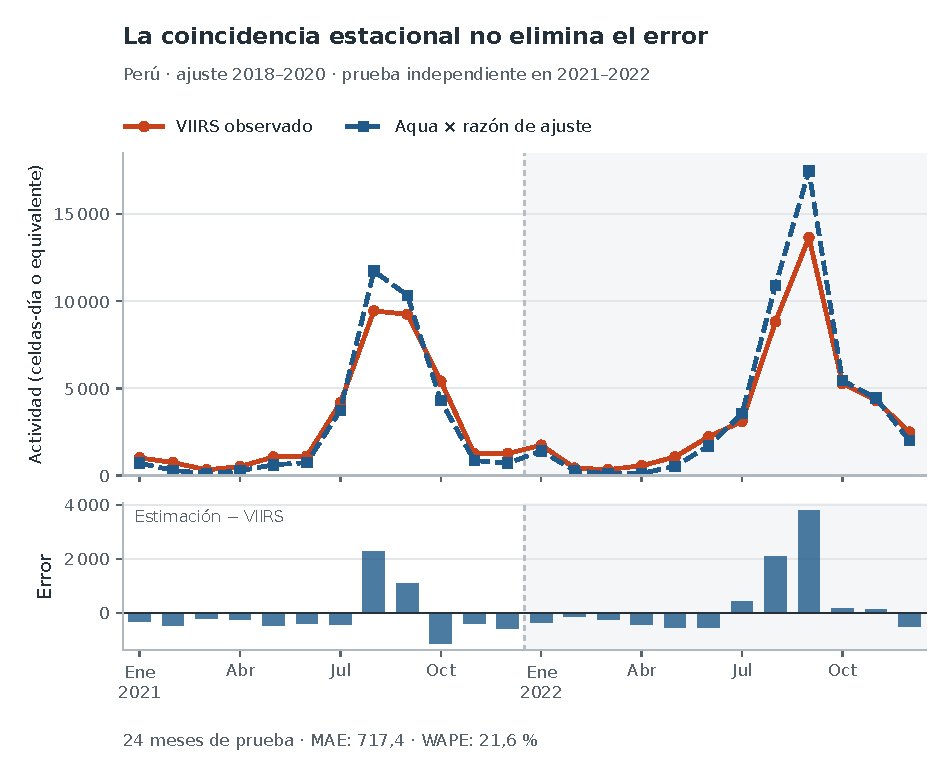
\includegraphics[width=\textwidth]{figuras/peru_validacion.pdf}
\caption{Validación temporal real en Perú. La razón se ajustó con 2018--2020 y se aplicó
sin cambios a los 24 meses de 2021--2022. Una buena coincidencia del ciclo estacional
no garantiza que coincidan las amplitudes mensuales. El panel inferior muestra el error
firmado: por encima de cero la conversión sobreestima el registro VIIRS; por debajo,
lo subestima.}
\label{fig:peru-validacion}
\end{figure}

El MAE de prueba es \PeruMAE{} unidades mensuales y el sesgo medio es
$+\PeruSesgo{}$. Para expresar un error relativo sin dividir cada mes por su propio
conteo, usamos
\begin{equation}\label{eq:wape}
 \mathrm{WAPE}=100\frac{\sum_m|\widehat V_m-V_m|}{\sum_m V_m},\qquad \sum_m V_m>0.
\end{equation}
Resulta \PeruWAPE{} por ciento. Esta medida da más influencia a los meses de gran
actividad. No afirma que cada mes tenga ese porcentaje de error; se acompaña del
gráfico de residuos y del MAE. Si todos los valores observados son cero, tampoco WAPE
está definido.

\begin{atencion}[El resultado real no se maquilla]
La razón única captura parte de la relación, pero deja desacuerdos apreciables. No
ajustamos el factor con los años de prueba para que las curvas queden bonitas. Un paso
posterior podría estudiar estratos regionales o estacionales, cobertura y estabilidad
temporal. Habría que seleccionar esas variantes con validación interna y evaluarlas en
otros años reservados. Este resultado es una línea base reproducible.
\end{atencion}

La diferencia entre los dos totales anuales puede ser pequeña por cancelación de
errores mensuales. Sobreestimar agosto y subestimar septiembre puede dejar un año casi
perfecto mientras arruina el calendario operativo. Por eso se evalúa en la resolución
temporal para la que se quiere usar el producto.

\FloatBarrier
\section{Segundo experimento: la razón no es constante}\label{sec:peru-modelos}

El panel de errores de la figura~\ref{fig:peru-validacion} no es ruido: la conversión
sobreestima los meses de más actividad y subestima los de menos, los dos años. Un error
con forma indica que al modelo le falta algo. El capítulo~\ref{cap:deteccion} anticipa
qué: fuera de temporada predominan fuegos pequeños, que Aqua casi no registra, y la razón
entre sensores debería ser mayor.

Para comprobarlo se calcula la razón de sumas de cada mes del año con los tres años de
ajuste (figura~\ref{fig:peru-razon-mensual}). Va de \PeruRazonMin{} en septiembre a
\PeruRazonMax{} en marzo: cambia más de tres veces a lo largo del año. La razón única de
\PeruRatio{} es, en la práctica, la razón de agosto y septiembre, porque esos dos meses
aportan dos tercios de las celdas-día de Aqua.

\begin{figure}[!htbp]
\centering
\begin{tikzpicture}
\begin{axis}[width=13cm,height=6.2cm,ybar,bar width=14pt,ymin=0,ymax=13,
  xmin=0.3,xmax=12.7,xtick={1,...,12},xticklabels={E,F,M,A,M,J,J,A,S,O,N,D},
  ylabel={Razón Suomi NPP / Aqua},axis lines*=left,ymajorgrids,grid style={ceniza!20},
  nodes near coords,nodes near coords style={font=\scriptsize,/pgf/number format/.cd,fixed,precision=1,use comma},
  ]
\addplot[fill=fuego!70,draw=none] table[x=mes,y=razon]{datos/peru_razon_mensual.dat};
\draw[cielo,very thick,dashed] (axis cs:0.3,4.685)--(axis cs:12.7,4.685);
\node[cielo,font=\footnotesize,anchor=north east] at (axis cs:12.6,12.8) {línea discontinua: razón única, 4{,}7};
\end{axis}
\end{tikzpicture}
\caption{Razón de sumas entre celdas-día de Suomi NPP y de Aqua para cada mes del año, Perú,
2018--2020. Datos reales. En marzo la razón se apoya en solo 119 celdas-día de Aqua en tres
años, de modo que su valor es incierto; la tendencia general no lo es.}
\label{fig:peru-razon-mensual}
\end{figure}

\subsection{Cuatro modelos y una regla para elegir}

Se comparan cuatro formas de convertir Aqua en Suomi NPP, todas del
capítulo~\ref{cap:estadistica}:

\begin{itemize}
  \item \textbf{razón única}: $\widehat V = r\,A$;
  \item \textbf{razón trimestral}: una razón para cada trimestre del año;
  \item \textbf{razón mensual}: una razón para cada mes del año;
  \item \textbf{ley de potencia}: $\widehat V = \alpha A^{\beta}$, ajustada por mínimos
  cuadrados sobre los logaritmos de los 36 meses de ajuste.
\end{itemize}

El modelo no puede elegirse mirando 2021--2022: eso convertiría la prueba en parte del
ajuste. La elección se hace con \emph{validación cruzada} dentro de 2018--2020: se aparta
un año, se ajusta con los otros dos, se predice el año apartado, y se repite con cada
uno de los tres. El modelo con menor WAPE en esa validación interna se evalúa después,
una sola vez, en los años de prueba.

\begin{table}[ht]
\centering
\begin{tabular}{lrrrr}
\toprule
 & Selección & Prueba & \multicolumn{2}{c}{Contraste} \\
\cmidrule(lr){2-2}\cmidrule(lr){3-3}\cmidrule(lr){4-5}
Modelo & validación cruzada & 2021--2022 & 2013--2017 & 2023--2024 \\
\midrule
Razón única & \PeruCVUnica & \PeruTestUnica & \PeruAntesUnica & \PeruDespuesUnica \\
Razón trimestral & \PeruCVTrim & \PeruTestTrim & \PeruAntesTrim & \PeruDespuesTrim \\
Razón mensual & \PeruCVMens & \PeruTestMens & \PeruAntesMens & \PeruDespuesMens \\
Ley de potencia & \textbf{\PeruCVPot} & \textbf{\PeruTestPot} & \PeruAntesPot & \PeruDespuesPot \\
\bottomrule
\end{tabular}
\caption{WAPE mensual, en porcentaje, de cuatro modelos de conversión de Aqua a Suomi NPP en
Perú. Datos reales. Todos los modelos se ajustan con 2018--2020. Los periodos de contraste
tienen otra etiqueta de versión en los archivos MODIS (\texttt{6.2} y \texttt{61.03}), por lo
que son una comprobación adicional y no una validación homogénea.}
\label{tab:peru-modelos}
\end{table}

La validación cruzada elige la ley de potencia, con
\begin{equation}
  \widehat V = \PeruPotAlfa\;A^{\,\PeruPotBeta}.
\end{equation}
En los años de prueba su WAPE es \PeruPotWAPE{} por ciento, frente a \PeruWAPE{} de la razón
única: el error se reduce a un tercio, el MAE baja de \PeruMAE{} a \PeruPotMAE{} y el sesgo
de $+\PeruSesgo$ a $+\PeruPotSesgo$ (figura~\ref{fig:peru-modelos}).

\begin{figure}[!htbp]
\centering
\begin{tikzpicture}
\begin{axis}[width=13.5cm,height=7cm,xmin=0.5,xmax=24.5,ymin=0,ymax=19000,
  xtick={1,4,7,10,13,16,19,22},xticklabels={ene 21,abr,jul,oct,ene 22,abr,jul,oct},
  ylabel={Celdas-día mensuales},scaled y ticks=false,
  y tick label style={/pgf/number format/1000 sep={\,}},
  legend style={at={(0.03,0.96)},anchor=north west,font=\small,draw=ceniza!40},
  grid=major,grid style={ceniza!15}]
\addplot[black,very thick,mark=*,mark size=1.6pt] table[x=t,y=viirs]{datos/peru_modelos_prueba.dat};
\addplot[cielo,thick,dashed,mark=square*,mark size=1.4pt] table[x=t,y=unica]{datos/peru_modelos_prueba.dat};
\addplot[fuego,very thick,mark=triangle*,mark size=1.8pt] table[x=t,y=potencia]{datos/peru_modelos_prueba.dat};
\legend{Suomi NPP observado,Aqua con razón única,Aqua con ley de potencia}
\end{axis}
\end{tikzpicture}
\caption{Los 24 meses de prueba con los dos modelos extremos de la
tabla~\ref{tab:peru-modelos}. Datos reales. La razón única exagera los picos de agosto y
septiembre; la ley de potencia los sigue de cerca.}
\label{fig:peru-modelos}
\end{figure}

\subsection{Cómo leer el exponente}

Un exponente $\beta = \PeruPotBeta$, menor que 1, dice que cuando la actividad registrada
por Aqua se duplica, la de Suomi NPP se multiplica solo por $2^{\PeruPotBeta} \approx 1{,}68$.
La razón entre sensores no es una constante del instrumento: disminuye cuando hay más fuego.
Es coherente con dos mecanismos ya estudiados. En plena temporada hay fuegos mayores, que
ambos sensores detectan. Y la celda-día satura: una celda con actividad intensa ya cuenta
<<uno>> para los dos.

La ley de potencia gana a la razón mensual aunque usa dos parámetros y no doce. La razón
mensual supone que cada agosto se parece a los demás agostos; la ley de potencia responde
al nivel de actividad del mes concreto, sea cual sea su fecha.

\subsection{Por región natural}

El último paso separa el país en costa, sierra y selva. No se dispone aquí del mapa oficial
de regiones naturales, así que se usa una regla de relieve sobre un modelo de elevación
público (teselas Terrarium, unos 2~km por píxel): una celda es \emph{sierra} si su elevación
media es de al menos 2000~m o si queda encerrada entre cumbres de su misma latitud; es
\emph{costa} si está por debajo de 2000~m al oeste de la cordillera, y \emph{selva} si lo está
al este. La regla coloca bien siete ciudades de control (Lima y Piura en la costa; Huancayo y
Cusco en la sierra; Pucallpa, Iquitos y Puerto Maldonado en la selva), pero asigna a la
<<costa>> las laderas occidentales bajas y a la <<selva>> toda la ceja de selva por debajo de
2000~m. Es una aproximación declarada.

\begin{table}[ht]
\centering
\begin{tabular}{lrrrrrr}
\toprule
 & \multicolumn{2}{c}{Celdas-día 2018--2020} & Razón & Exponente & \multicolumn{2}{c}{WAPE 2021--2022} \\
\cmidrule(lr){2-3}\cmidrule(lr){6-7}
Región & Aqua & Suomi NPP & única & $\beta$ & razón única & potencia \\
\midrule
Costa & \RegCostaAqua & \RegCostaVIIRS & \RegCostaRazon & \RegCostaBeta & \RegCostaWapeUnica & \RegCostaWapePot \\
Sierra & \RegSierraAqua & \RegSierraVIIRS & \RegSierraRazon & \RegSierraBeta & \RegSierraWapeUnica & \RegSierraWapePot \\
Selva & \RegSelvaAqua & \RegSelvaVIIRS & \RegSelvaRazon & \RegSelvaBeta & \RegSelvaWapeUnica & \RegSelvaWapePot \\
\bottomrule
\end{tabular}
\caption{Calibración de Aqua a Suomi NPP por región natural aproximada. Datos reales. Cada
región se ajusta por separado con 2018--2020 y se prueba en 2021--2022. Las tres regiones
suman exactamente el total nacional de la tabla~\ref{tab:peru-ajuste}.}
\label{tab:peru-regiones}
\end{table}

Tres lecturas de la tabla~\ref{tab:peru-regiones}.

\textbf{La razón cambia con la región.} En la costa Suomi NPP registra \RegCostaRazon{} veces
más celdas-día que Aqua; en la selva, \RegSelvaRazon. Aplicar la razón nacional de \PeruRatio{}
a la costa la subestimaría casi a la mitad. Es lo que se espera donde las quemas son pequeñas
y Aqua apenas las registra.

\textbf{La ley de potencia mejora en las tres regiones}, aunque de forma desigual: mucho en la
selva y en la costa, poco en la sierra.

\textbf{Con menos datos, más error.} La costa aporta solo \RegCostaAqua{} celdas-día de Aqua en
tres años; sus parámetros son los menos seguros. Es la advertencia de la
ecuación~\eqref{eq:rel} con números reales.

Si se suman las tres conversiones regionales y se comparan con el total nacional observado,
el WAPE mensual es \RegSumaUnica{} por ciento con razones únicas regionales (frente a
\PeruWAPE{} de la razón nacional) y \RegSumaPot{} por ciento con leyes de potencia regionales
(frente a \PeruPotWAPE{} de la ley nacional). Estratificar ayuda mucho a la razón única y no
mejora el total nacional de la ley de potencia; lo que aporta en ese caso es una serie
convertida para cada región, que es lo que necesita un usuario que elige un área.

\subsection{El eslabón hacia el presente: de Suomi NPP a NOAA-20}\label{sec:peru-noaa20}

Suomi NPP dejó de entregar datos nuevos el 2 de noviembre de 2026. Una serie calibrada en su
escala necesita un sucesor para seguir creciendo, y el natural es NOAA-20: el mismo instrumento
en la misma órbita de las 13:30, unos 50 minutos por detrás. Es el segundo eslabón de la cadena
de la figura~\ref{fig:cadena}, y mucho más sencillo que el primero.

Se descargaron los archivos nacionales de NOAA-20 (carpeta \texttt{viirs-jpss1} de FIRMS) de
2018 a 2025, todos con etiqueta de versión \texttt{2}, y se procesaron con los mismos filtros. El
diseño se fijó antes de ver los resultados: ajuste con 2019--2021 y prueba con 2022--2024. El año
2018 queda fuera porque sus datos empiezan el 1 de abril, cuando el satélite entró en servicio.

En los años de ajuste, Suomi NPP registra \NveinteAjusteSNPP{} celdas-día y NOAA-20
\NveinteAjusteNveinte, de modo que
\begin{equation}
  \widehat{V}_{\text{SNPP}} = \NveinteRazon\;V_{\text{NOAA-20}} .
\end{equation}
Ajustada sobre los logaritmos, la ley de potencia da $\beta = \NveinteBeta$: proporcionalidad
pura. Entre dos copias del mismo instrumento en la misma órbita la relación no depende del nivel
de actividad, al revés de lo que ocurre entre Aqua y Suomi NPP.

En los 36 meses de prueba, usar NOAA-20 sin convertir ya da un WAPE de \NveinteWapeSin{} por
ciento; con la razón baja a \NveinteWapeRazon{} por ciento, con un sesgo medio de
$+\NveinteSesgoRazon$ celdas-día por mes. La ley de potencia no añade nada
(\NveinteWapePot{} por ciento), y por el principio de preferir el modelo más simple se usa la
razón.

Con este eslabón, la serie continúa en 2025: NOAA-20 registra \NveinteTotalVeinticinco{}
celdas-día, equivalentes a \NveinteConvVeinticinco{} en escala Suomi NPP. Es el valor más bajo
de todo el registro, con agosto y septiembre en torno a la mitad de lo habitual. Los datos no
dicen por qué; antes de interpretarlo habría que descartar cambios de cobertura o de
procesamiento en ese año.

\begin{parareto}
La cadena completa queda así: los años de Aqua se llevan a escala Suomi NPP con la ley de
potencia; desde 2025, NOAA-20 se lleva a la misma escala multiplicando por \NveinteRazon. El
error del segundo eslabón (\NveinteWapeRazon{} por ciento) es pequeño frente al del primero, de
modo que la incertidumbre de la serie la domina la conversión de MODIS. Y si NOAA-20 falla, el
mismo procedimiento sirve para NOAA-21.
\end{parareto}

\begin{atencion}[Corrección posterior: había cortes de servicio en estos años]
Una auditoría hecha después de escribir este capítulo encontró que los años elegidos contienen
periodos en que un satélite no observó. Aqua estuvo sin datos del 16 de agosto al 2 de
septiembre de 2020 (en esa quincena la razón entre sensores es 26, frente a 3--4 en los demás
años) y del 31 de marzo al 16 de abril de 2022. Suomi NPP estuvo en modo seguro del 26 de julio
al 10 de agosto de 2022. Los archivos de focos no avisan de estos cortes: el de Aqua de 2020 ni
siquiera deja días vacíos, porque se reprocesó con cobertura parcial.

Repitiendo el ejercicio nacional sin los seis meses afectados (agosto y septiembre de 2020;
marzo, abril, julio y agosto de 2022), la razón única baja de \PeruRatio{} a 4,541 y la ley de
potencia queda en $\widehat V = 29{,}5\,A^{0{,}73}$. En la prueba, el WAPE es 19,6 por ciento
con la razón única y 7,4 por ciento con la ley de potencia. La conclusión no cambia: la ley de
potencia reduce el error a menos de la mitad. Los valores de las tablas de esta sección se
conservan tal como se calcularon, con los cortes dentro.

La lección es de método: \textbf{antes de calibrar dos sensores hay que comprobar que ambos
estaban observando}. La forma de hacerlo es comparar sus conteos diarios y buscar periodos en
que uno cae sin que caiga el otro. El análisis corregido, con relleno de los cortes de Suomi
NPP mediante NOAA-20, está en \texttt{proyecto/docs/METODOS.md}.
\end{atencion}

\begin{atencion}[Lo que este resultado no demuestra]
\begin{itemize}
  \item Es un ajuste \textbf{nacional y mensual}. A la escala de una provincia o de una
  semana, con conteos mucho menores, los parámetros pueden ser otros y el error será mayor.
  \item Una ley de potencia con $\beta<1$ \textbf{no es aditiva}: convertir cada provincia
  y sumar no da lo mismo que convertir el total nacional. Hay que ajustarla en la misma
  escala en la que se va a aplicar.
  \item En 2023--2024 el error sube a \PeruDespuesPot{} por ciento. Puede deberse al cambio
  de etiqueta de versión, a la deriva orbital de Aqua (capítulo~\ref{cap:orbitas}) o al azar
  de dos años; con estos datos no se puede distinguir.
  \item Sigue siendo una comparación entre sensores sin corrección de nubes ni de cobertura.
\end{itemize}
\end{atencion}

\begin{parareto}
Este es un resultado propio y verificable para la presentación: \emph{en Perú, la relación
entre MODIS y VIIRS depende del nivel de actividad; modelarla con una ley de potencia reduce
el error de conversión mensual de \PeruWAPE{} a \PeruPotWAPE{} por ciento en años no usados
para el ajuste}. Se reproduce con \texttt{scripts/comparar\_modelos.py} y
\texttt{scripts/regiones\_peru.py}. Un segundo mensaje: la razón de la costa es el doble que
la de la selva, así que un factor nacional único perjudica a las regiones con menos fuego.
\end{parareto}

\FloatBarrier
\section{Una interfaz que permita verificar}

La primera vista puede responder tres preguntas: \emph{dónde}, \emph{cuándo} y
\emph{comparado con qué}. Un mapa define el área; un calendario muestra los periodos;
una curva enseña la referencia histórica. La selección de un mes debe actualizar las
tres vistas de forma consistente.

Al acercarse a un lugar conviene mostrar una imagen real del terreno y, por separado,
la capa de detecciones. El ejemplo del Camp Fire del capítulo~\ref{cap:problema} explica
visualmente por qué un punto no es el contorno del incendio. La escena peruana del
capítulo~\ref{cap:atmosfera} recuerda que una imagen vistosa puede tener mucho suelo
oculto. Las imágenes ayudan a interpretar la medición; no reemplazan la definición
del indicador.

Cada detalle debe mostrar fecha, sensor, unidad, filtros y estado de calidad. Una
casilla sin observación conocida debe distinguirse de una casilla con cero detecciones,
por ejemplo con una trama y una etiqueta, sin depender solo del color. Las escalas
entre áreas comparadas deben ser iguales o explicitar que cambiaron. Un rojo significa
un valor en una escala, no necesariamente peligro.

Es útil ofrecer la comparación entre series originales y convertidas. Ocultar las
originales vuelve imposible ver qué parte del cambio proviene del sensor y qué parte
del método. Para exportar una figura, su pie debe incluir el periodo de referencia y
la fecha de actualización; para exportar una tabla, debe incluirse el identificador
de la versión del análisis.

\FloatBarrier
\section{Comprobaciones que detectan errores reales}

Las verificaciones útiles comprueban propiedades del problema. Si una fila aparece
dos veces de forma idéntica, no debe cambiar la presencia diaria. Si una detección
se mueve de las 23:59 a las 00:01 UTC, hay que comprobar qué pasa con su fecha local.
Si cambian la rejilla o el sensor, la caché no debe reutilizar la respuesta anterior.
Si el denominador de una anomalía es cero, la pantalla debe mostrar un estado definido.

La validación científica añade preguntas diferentes: ¿se mantiene el error fuera del
periodo de ajuste?, ¿cambia por mes?, ¿la razón es estable cuando cambia la versión o
la hora de paso?, ¿una fuente térmica persistente domina una zona? Pasar pruebas de
software demuestra que el programa cumple sus reglas, no que esas reglas representen
adecuadamente el fenómeno.

\begin{parareto}[Una demostración defendible]
Muestra una región peruana, su calendario y una escena real. Explica la unidad, enseña
la comparación de sensores y los años reservados para validación. Después señala una
limitación concreta y cómo se refleja en la interfaz. El valor del proyecto está en
que otra persona pueda comprender, reproducir y discutir esa cadena de decisiones.
\end{parareto}

\FloatBarrier
\section{Cómo reproducir el caso del libro}

Desde la carpeta del libro se ejecutan:
\begin{lstlisting}
bash scripts/descargar_peru.sh
python3 scripts/analizar_peru.py
python3 scripts/verificar_ejemplos.py
python3 scripts/generar_graficos.py
latexmk -pdf -interaction=nonstopmode -halt-on-error libro.tex
\end{lstlisting}
La primera orden conserva los archivos ya existentes. Las siguientes calculan las
tablas, comprueban ejemplos aritméticos y compilan. Los CSV originales ocupan alrededor
de 84 MiB en esta descarga. El análisis usa únicamente la biblioteca estándar de
Python. La generación de las cuatro figuras vectoriales del caso peruano usa Matplotlib
y NumPy; la compilación requiere los paquetes LaTeX declarados en el preámbulo.

\path{datos/procedencia_peru.json} permite identificar los originales.
\path{datos/resultados_peru.json} conserva los filtros y cifras principales.
\path{datos/peru_mensual.csv} contiene las agregaciones, y
\path{datos/peru_validacion.csv}, las predicciones y errores de prueba. Las figuras leen
esas tablas mediante los scripts incluidos. Si el proveedor reprocesa un archivo, su huella cambia:
se conserva la versión anterior para distinguir una revisión de datos de un cambio
en el método.

\resumen
\begin{itemize}
\item Preservar originales, normalizar observaciones y materializar indicadores permite
reproducir una cifra y localizar el origen de un cambio.
\item La unión de presencias, la suma de celdas-día y el cambio de rejilla son operaciones
distintas; el modelo de datos debe conservar lo necesario para cada una.
\item Leer menos columnas y evitar trabajo repetido suele importar más que añadir núcleos.
\item La calibración peruana se ajustó con 2018--2020 y se probó con 2021--2022; su WAPE
mensual fue \PeruWAPE{} por ciento, bajo los filtros declarados.
\item La razón entre sensores no es constante: va de \PeruRazonMin{} a \PeruRazonMax{} según
el mes y de \RegSelvaRazon{} en la selva a \RegCostaRazon{} en la costa. Una ley de potencia
elegida por validación cruzada reduce el WAPE de prueba a \PeruPotWAPE{} por ciento.
\item El paso de Suomi NPP a NOAA-20 es proporcional (razón \NveinteRazon, WAPE
\NveinteWapeRazon{} por ciento) y permite continuar la serie después del cierre de Suomi NPP.
\item Una pantalla útil deja inspeccionar fuentes, incertidumbre y series originales.
\item Corrección del código y validez científica necesitan comprobaciones complementarias.
\end{itemize}

\ejercicios
\begin{enumerate}
\item Reconstruye la razón $124188/26508$ a partir de los CSV mensuales y comprueba el
MAE y el sesgo de los 24 meses de prueba.
\item Calcula el error anual de 2021 y de 2022. Compáralo con los errores mensuales y
explica qué información se pierde al publicar solo los totales anuales.
\item Si se convierten dos zonas con razones 2 y 5 y conteos 100 y 20, calcula el total
convertido. ¿En qué condiciones una sola razón produciría el mismo resultado?
\item Diseña una clave de caché para una consulta provincial. Indica qué partes cambian
si solo se modifica la paleta y cuáles si se actualiza el periodo de referencia.
\item Compara en memoria las claves guardadas como cadenas con una representación
entera compacta. Mide memoria y tiempo, y comprueba que las claves únicas coinciden.
\item Con la ley de Amdahl, calcula el límite de aceleración si solo el 60\,{}\% del
tiempo es paralelizable. ¿Qué ocurriría si la etapa serial se redujera a la mitad?
\item Diseña cuatro filas de entrada que prueben un duplicado idéntico, un borde de
celda, un cambio de día local y una clase de confianza desconocida.
\item Redacta el pie de una figura exportada para que siga siendo interpretable fuera
de la aplicación. Incluye unidad, fuente, periodo, selección y limitación principal.
\item Esboza una validación interna para elegir entre razón única y razones por
trimestre sin volver a usar los años de prueba para escoger el modelo.
\end{enumerate}

\lecturas
La documentación de Parquet y DuckDB explica las propiedades concretas del almacenamiento
columnar y de su ejecución.\fuente{parquet}\fuente{duckdb} El trabajo de Amdahl formaliza
el límite del paralelismo.\fuente{amdahl} Para practicar con las entradas reales de
FIRMS, sus materiales de formación describen la ingestión y la API.\fuente{firms-ingest}\fuente{firms-api}
